% Design 
%!TEX root = ../Project.tex
\section{Design}

\subsection{Methodologies}
\label{sub:methodologies}
The Model View Controller (MVC) design paradigm was chosen to be used to structure the project. The MVC design patten has many benefits, as discussed below.  

Firstly the MVC patten divides the engine into three logical components, namely the model the controller and the view.  

The model is where the game state is stored, containing all the relevant data relating to the players in the game and the game itself.  The controller contains the code to handle  the manipulation of the model and data conversion.

\subsubsection{Advantages of MVC for this project}
\label{ssub:advantages_of_mvc_for_this_project}

The domain separation that the MVC pattern gives is useful as it encourages loose coupling between the representation of the data and the data itself. This is useful for this project since it allowed the creation of new views, using the same model. This easily supports future developments such as a mobile version of the engine.

\subsection{Engine}
The main considerations  for the engine was to make it as configurable as possible. To achieve this everything was designed in terms of interfaces, which allowed the particular implementation to be changed. The objects themselves were loaded from their serialised form on disk. 

\subsubsection{Data Format}
\label{ssub:data_format}
XMl was chosen as the data format for this project. The main reason is that it is human readable, this allowed me to create and test the data format before the editor was created.

The data was designed to be extendable, as well as provide implementations of the various assets. An advanced user can specify their own custom classes.

\begin{lst:weapon}[caption=Example of Custom weapon, label=lst:weapon]
<weapon class="custom.customWeapon" uuid="0f0dee33">
	<name>Longicolnis</name>
</weapon>
\end{lst:weapon}

Listing \ref{lst:weapon} shows how a custom weapon can be used. The \texttt{class} attribute is  the fully qualified name of the class. The only thing the user has to do is to add a \texttt{jar} with their classes in it to the \texttt{classpath} of the game. 

\subsubsection{XML schema}

XML schema is a way of validating an  xml document. A schema was produced for each serialised object\footnote{in the \texttt{schemas} directory}. 
The main use of this was for testing the hand written xml I used before the editor was created. It also helped ensure that the xml produced by the editor was correct.  

\subsection{Game Progression}
\begin{figure}[htbp]
	\centering
		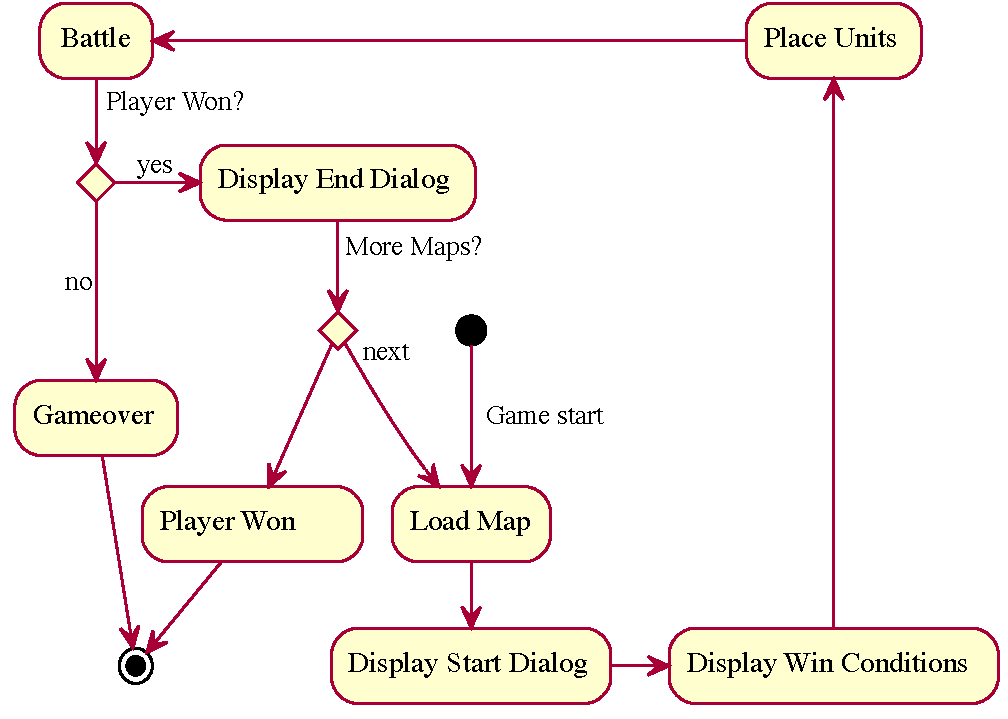
\includegraphics[height=3in]{figures/game.pdf}
	\caption{Activity diagram which a high level of overview of the engine}
	\label{fig:figures_game}
\end{figure}

Figure \ref{fig:figures_game} shows the overview of how the created game progresses.  Each game has a number of maps where a battles takes place. After the map is loaded, any relevant dialogue is displayed, along with the winning conditions. The player's units are then placed on the map, and the battle starts\footnote{While the engine allows the user to choose where their units are placed, the GUI does not due to time constraints. The editor supports specifying the starting location for the player's units.}. If the player loses the battle, a gameover screen is shown and the game ends. In contrast if the player wins, he/she advances to the next map, if there is one.    

\subsection{Game Mechanics}
As apparent from the name of the project, a TRPG is turn-based.  There were two main choices for turns works; the first is where the players take turns to move all the units, the other method is where the next unit to move is based on some statistic such as the unit's agility. Both methods are widely used,  the first more often in games that focus on micro-management such as \emph{Civilization} but there are exceptions to this such as \emph{Disgaea}. 

The second method has the advantage of allowing more dynamic unit ordering.  An example of how this is commonly used: A unit can get their turn quicker if they did not perform any action on their last turn. It also has the advantage of making the game flow much quicker, since the player does not have to wait too long to move their next unit. 

I chose to use the second method because it allows the user more customisability since they can choose how unit ordering works. The other reason is based on my own experience, where I think it works better.

\subsection{Map Rendering}

\subsubsection{Introduction}
An isometric viewpoint is a way of display 3d objects in 2d while giving the impression that it s 3d.  Two different variations are shown in figure \ref{fig:tilemap0}.  

The main benefit of an isometric map compared to a topdown view is that height can be easily displayed. 

\subsubsection{Tilemap}
\label{sub:tilemap}

There were two main choices for the isometric tilemap, a ``Diamond'' map or a  ``Staggered'' map \cite{isometric_game_programming}, examples of both are shown below in figure \ref{fig:tilemap0}. Prototypes of each map type were created and the following was found.  

The ``Staggered'' was the first to be considered and it had the following advantages:
\begin{itemize}
	\item The map filled up the screen with very little wasted space, so the user can see more of what is happening on the map. 
\end{itemize}

The ``Diamond'' map was chosen for the following reasons:
\begin{itemize}
	\item ``Diamond'' map look more aesthetically pleasing than ``Staggered'' maps because it has no ragged edges.
	\item  If the map is large enough, it will fill the whole screen negating the ``Staggered'' map advantage.
	\item  Simpler to think about, since a ``Diamond'' map is just a rectangular map rotated.
\end{itemize}


\def\tilemapSize{3in}
\begin{figure}[htbp]
	\begin{center}

	\subfigure[Diamond Map]{
		\label{fig:tilemap1} 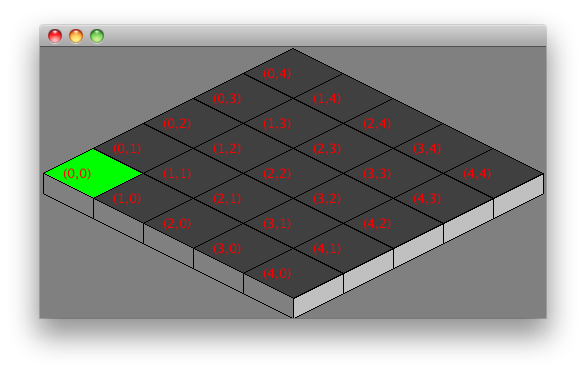
\includegraphics[width=\tilemapSize]{figures/tilemap1.png}} 
	\subfigure[Staggered Map]{
		\label{fig:tilemap2} 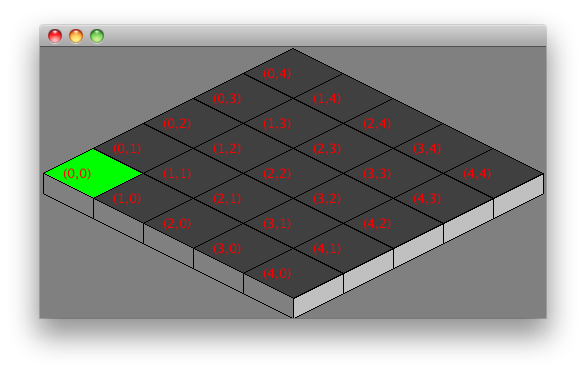
\includegraphics[width=\tilemapSize]{figures/tilemap2.png}} 
	\caption{\label{fig:tilemap0} The two main types of isometric tilemaps}
	\end{center}
\end{figure}

\clearpage

\subsection{Units}
\label{ssub:unit}
I designed the actions a unit can take as a finite state machine as show in figure \ref{fig:figures_unit}.  The main actions the unit can take are:
\begin{itemize}
	\item[\textbf{Move}]   This allows the unit to move to any tile in it's movement range.
	\item[\textbf{Attack}] Attack any opponent in their weapons range.
	\item[\textbf{Skill}]  Use one of their skills
	\item[\textbf{Wait}]   Finish their turn  without taking any action.
\end{itemize}

\begin{figure}[h]
	\centering
		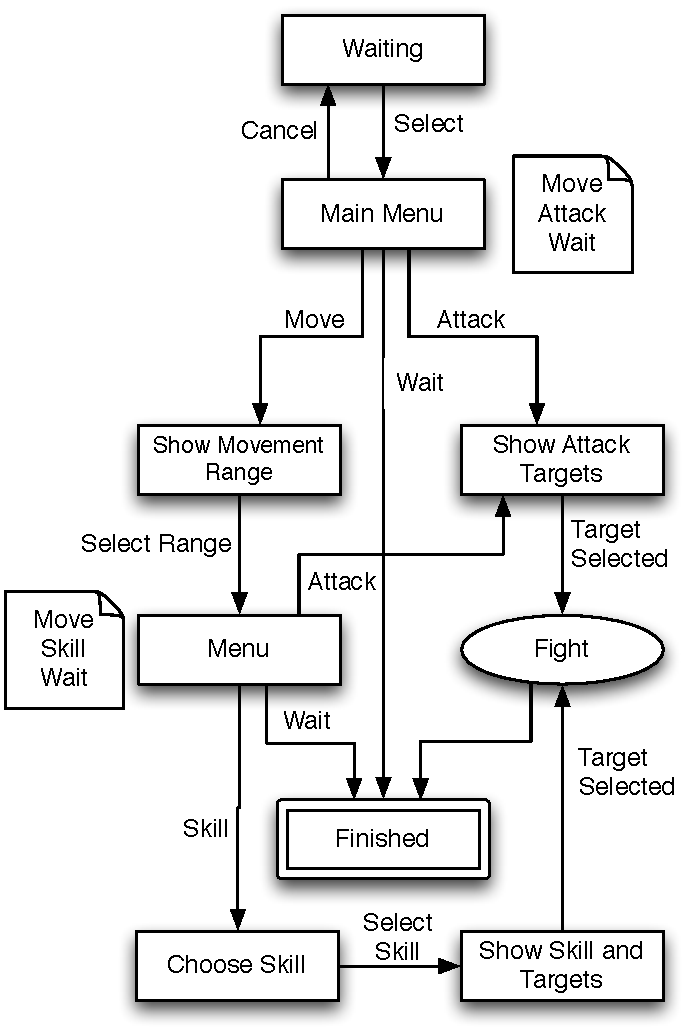
\includegraphics[width=4in]{figures/unit.pdf}
	\caption{The State diagram of a single turn of a player's unit}
	\label{fig:figures_unit}
\end{figure}

\clearpage
\subsection{Weapons \& Skills}
\label{sub:weapons___skills}



As is common in TRPG, I included weapons as  well as skills in the design.  A Weapon has a certain strength, a specified range and it may have unique effects.  As discussed in  section \ref{ssub:data_format},  the weapons and skills are completely configurable, but to enable the user to create common weapons, I designed the following weapons to be included as standard in the engine.  

\def\weapon{0.44}
\begin{figure}[htbp]
	\begin{center}
	\subfigure[Melee Weapon]{
		\label{fig:weapon1} 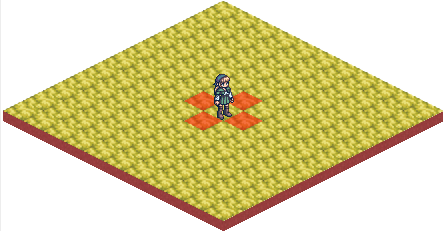
\includegraphics[scale=\weapon]{figures/weapon-melee.png}} 
	\subfigure[Spear]{
		\label{fig:weapon2} 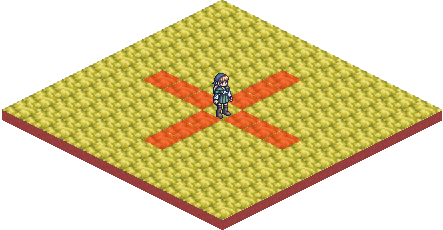
\includegraphics[scale=\weapon]{figures/weapon-spear.png}} 
	\subfigure[Ranged Weapon]{
		\label{fig:weapon3} 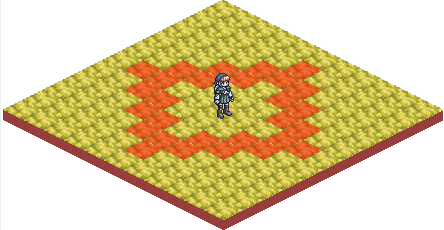
\includegraphics[scale=\weapon]{figures/weapon-ranged.png}} 
	\subfigure[Ranged Skill]{
		\label{fig:weapon4} 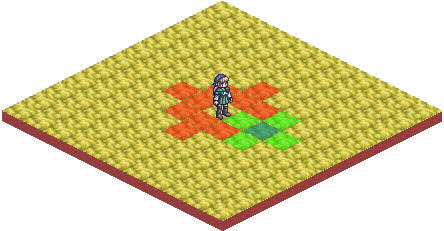
\includegraphics[scale=\weapon]{figures/skill.png}}		
	\caption{The above figure shows the attack range of various weapons and skill }
	\label{fig:weapons}
	\end{center}
\end{figure}

\paragraph{Melee Weapon} this is the simplest kind of weapon, where the unit can only attack adjacent enemies.

\paragraph{Spear} A spear can attack  enemies in it's range, in a single direction. The unique feature is that it damages \texttt{all} enemies in that direction at the same time.

\paragraph{Ranged Weapon} A ranged weapon attacks a single faraway target. It has the limitation of not been able to attack enemies which are too close (as shown in the diagram). 

\paragraph{Ranged Skill} A skill can attack  enemies in it's range. The main difference from a weapon is that the skill has an \texttt{attack area}(shown in green) which are the units affected. Unlike most weapons, skills affect \emph{all} units in the \texttt{attack area}.

\clearpage
\subsection{Editor}
The editor was designed to be easy to use. I designed a tabbed interface which allows the user to choose which parts to edit.  One of the main features of the editor is the updating of related panels. For example, if the user creates a new weapon, it will automatically be added to the list of available weapons. 
The main components of the editor are shown below.

\paragraph{Weapons \& Skills} the editor is designed to allow the user to visually see how changing the stats affect it. This includes showing the user the attack range of the weapon/skill.

\def\editor{0.23}
\begin{figure}[htbp]
	\begin{center}
	\subfigure[Weapons Panel]{
		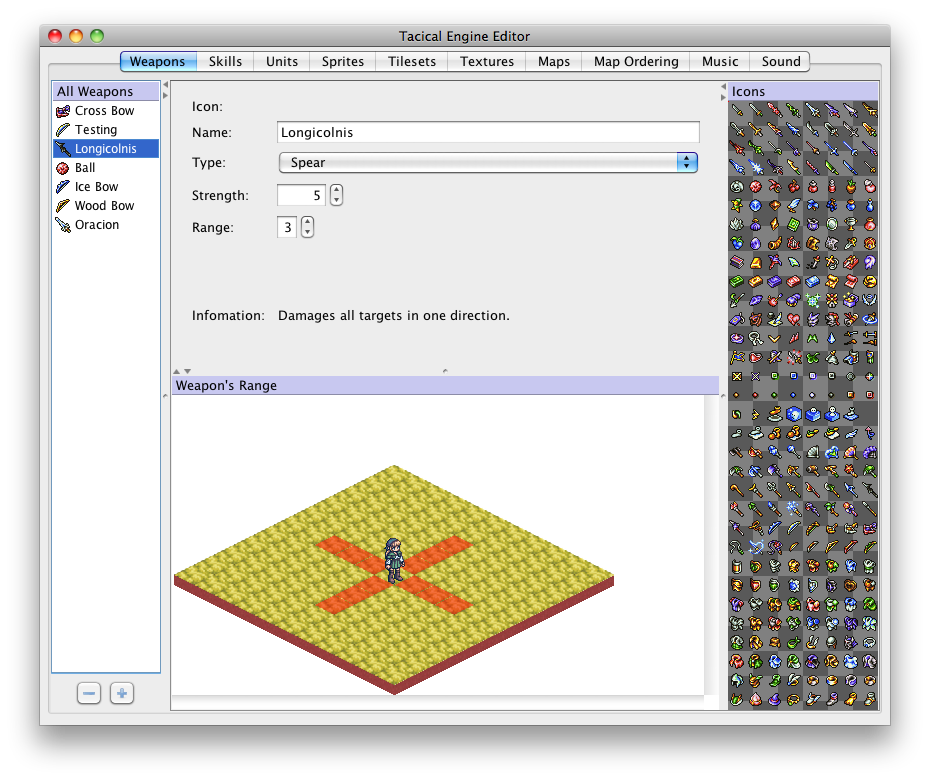
\includegraphics[scale=\editor]{figures/editor/Weapons.png}}
	\subfigure[Skill Panel]{
			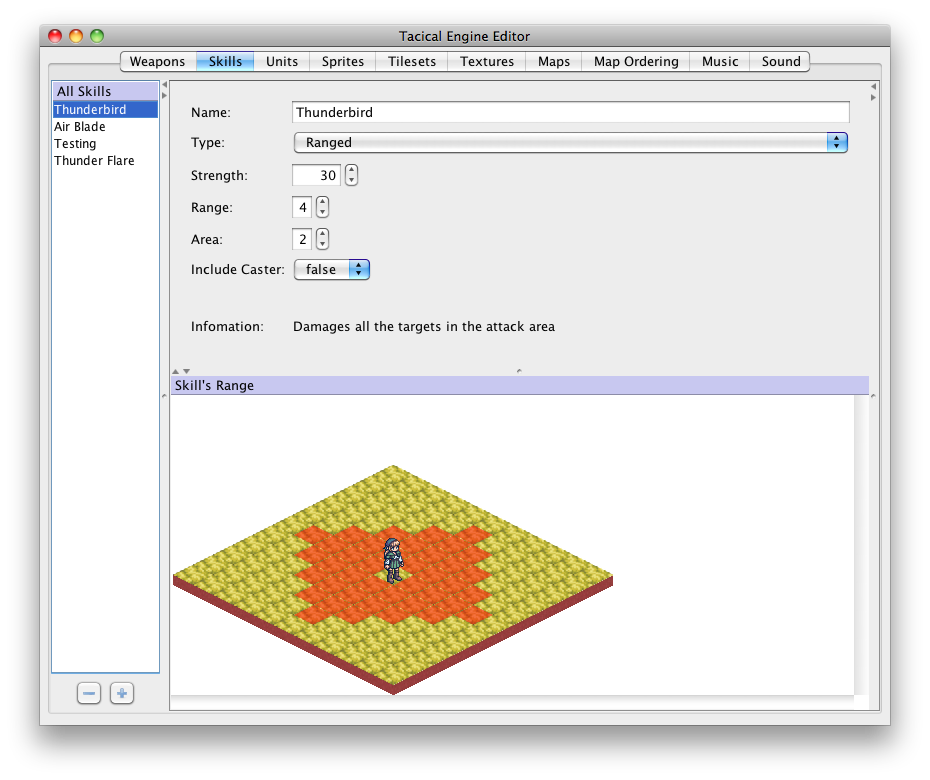
\includegraphics[scale=\editor]{figures/editor/Skills.png}}
	\end{center}
	\label{fig:editor}
\end{figure}

\paragraph{Units} All the attributes of the units are user editable. This includes their weapon, skill as well as the unit's sprites. 

 \begin{figure}[htbp]
 	\centering
 		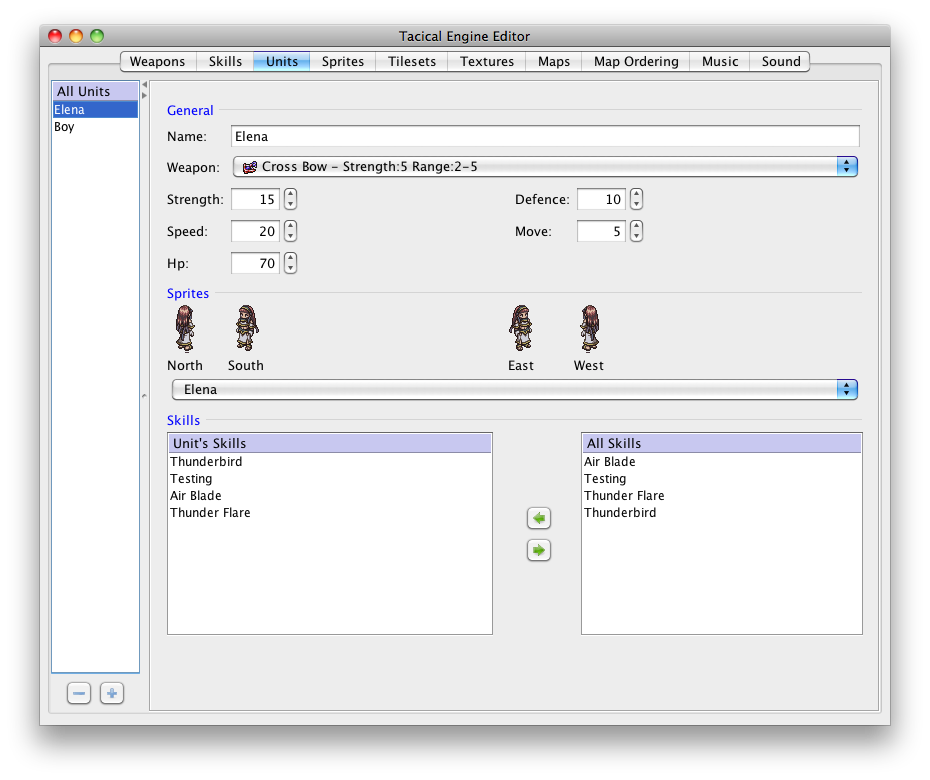
\includegraphics[scale=0.3]{figures/editor/Units.png}
 	\caption{Unit panel}
 	\label{fig:figures_editor_Unitsd}
 \end{figure}
 
\clearpage
\subsubsection{Visual Map Editing}
The editor supports visual map editing as shown in figure \ref{fig:figures_editor_Map}.  This allows the user to design their map without writing lots of xml. One of the notable features is that the user can specify the enemy's locations, which gives the user more freedom, compared with older TRPG where the enemies always start on the same corner on every map.  

\begin{figure}[htbp]
	\centering
		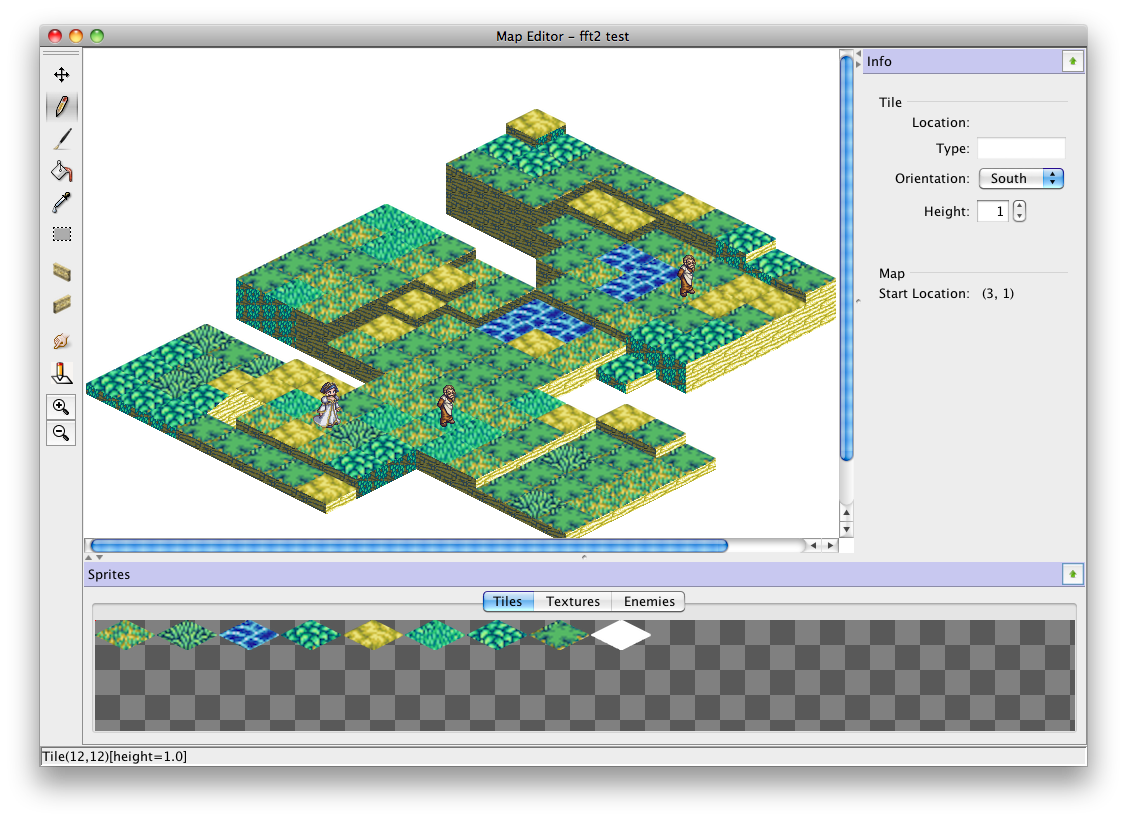
\includegraphics[height=5in]{figures/editor/Map.png}
	\caption{Visual Map Editor}
	\label{fig:figures_editor_Map}
\end{figure}

Each tile has many attributes associated with it, these include 
\begin{itemize}
	\item The main image.
	\item The left and right wall images.
	\item A specified height.
	\item An \emph{orientation}, which affects which way the slanted tiles are drawn.
\end{itemize}

The tools are based on their equivalents in a painting program  and include a \texttt{pencil} for drawing the currently selected tile image onto the selected tile.  Other tools include enemy unit placement using an icon of a pointing finger. 



% TODO  spinner commit on type
